\section{Fundamentals of IP Networking and Internet Routing}
\label{s:fundamentals}

This section introduces the main ideas and concepts that are used as a basis for traditional wired Internet. Subection \ref{ss:ip} presents the key elements of the IP networking model, including addressing, forwarding and the notion of IP link. Subection \ref{ss:routing} describes the most relevant routing techniques used in the Internet, and subsection \ref{ss:irarq} overviews the Internet routing architecture, based on the notion of Autonomous System. A certain familiarity with the basics of computer networking is assumed, so no details are provided. This section mainly follows the classic manuals of Tanenbaum {\em et al.} \cite{tanenbaum}, Comer \cite{comer} and Perlman \cite{interconnections}. Interested readers are referred to these resources for further explanations. \ \\ \ \\
% Assumptions:
% - TCP/IP stack
%
%This chapter focuses on communication in layer 3 (internetworking) for multi-hop IP networks (partly) composed of wireless links. Protocols and devices operating at this layer enable communication between hosts not belonging to the same link. 
%
\subsection{The IP Networking Model}
\label{ss:ip}
%
The Internet Protocol (IP) defines the key elements enabling communication in an IP network. This section presents the IP addressing mechanism, the notion of IP link and the routing rule used by router in IP networks -- the {\em longest prefix match} criterion.
%
\paragraph{Addressing}

In an IP network, every \glslink{interface}{\em network interface} is assigned at least one {\bf IP address} that identifies unambiguously the \glslink{interface}{interface} in the network. The IP address format varies depending on the protocol version (32 bits for IPv4, 128 bits for IPv6, see Figure \ref{f:ipa}), but three elements  can be distinguished.

\begin{itemize}
\item The {\bf host identifier} is the set of bits that identifies the \glslink{interface}{interface} in the network.
\item The {\bf network prefix} is the set of bits that identifies the network to which the \glslink{interface}{interface} is attached.
\item The {\bf network mask} allows to obtain the network prefix and the host identifier from the IP address. 
\end{itemize}

\begin{remark}
The IP address of a network \glslink{interface}{interface} is both an {\em identifier} and a {\em locator} of the interface: it indicates {\em who} is (unambiguosly in the internetwork) the attached \glslink{interface}{interface} and {\em where} is it attached (to which network).
\end{remark}

\begin{figure}[htb]
\centering
{\small a) IPv4 addressing example: $192.168.0.1/24$}
\begin{eqnarray*}
\textrm{Mask (24):} 		& \underbrace{{\tt 11111111}.{\tt 11111111}.{\tt 11111111}}_{\textrm{netmask (24 bits)}}.{\tt 00000000} \\
\textrm{IP address:} 	& \underbrace{{\tt 11000000}.{\tt 10101000}.{\tt 00000000}}_{\textrm{network prefix}}.\underbrace{{\tt 00000001}}_{\textrm{host identifier}}
\end{eqnarray*}
{\small b) IPv6 addressing example: $2001:0DB8:02DE::0E13/64$}
\begin{eqnarray*}
\textrm{Mask (64):} 			& \underbrace{{\tt FFFF}:{\tt FFFF}:{\tt FFFF}:{\tt FFFF}}_{\textrm{netmask (64 bits)}}:{\tt 0000}:{\tt 0000}:{\tt 0000}:{\tt 0E13} \\
\textrm{IP address:} 	& \underbrace{{\tt 2001}:{\tt 0DB8}:{\tt 02DE}:{\tt 0000}}_{\textrm{network prefix}}:\underbrace{{\tt 0000}:{\tt 0000}:{\tt 0000}:{\tt 0E13}}_{\textrm{host identifier}}
\end{eqnarray*}
\caption{IP address structure, for IPv4 and IPv6.}
\label{f:ipa}
\end{figure}
%
%\begin{remark}
%In the context of an IP network, a routing table is a local database that maps IP prefixes (from packet destinations) to the networking \glslink{interface}{interface} and the IP address of the next hop (to which the packet should be sent).
%\end{remark}
%
Based on the information contained in IP addresses from the destination field of the IP header, routers and hosts are able to take decisions upon reception of an IP packet. Trivially, a host receiving an IP packet will accept it only in case that the destination IP address is itself\footnote{Or the destination address is a broadcast address or a multicast address to which the host has suscribed.} and drop it otherwise. A router receiving an IP packet over an \glslink{interface}{interface} will compare the network prefix of the destination IP address with the prefix of its own interface: if it does not match, it may forward it through another interface, according to the IP forwarding rule (see below). In case of forwarding, the router decreases the {\em Time-To-Live} field (or {\em hop-limit} for IPv6), to indicate that the corresponding packet has traversed one (more) router in its path to its destination. This leads to the notion of \glslink{ip-link}{\em IP link} (see Figure \ref{f:iplink}).
%
\begin{definition}[IP Link]
Two network interfaces, $x$ and $y$, are connected to the same {\em IP link} when they can exchange packets in an IP network without requiring that any router forwards them, that is, when packets sent from one \glslink{interface}{interface} are received in the other with the same TTL/hop-limit value. This relationship is denoted as $x \sim_{IP} y$.
\end{definition}
%
\begin{itemize}
\item In these conditions, communication is performed in a single {\em IP hop}.
\end{itemize}

%Let $\sim_{IP}$ denote the IP link relationship, by which $x \sim_{IP} y$ if and only if network interfaces $x$ and $y$ belong to the same IP link, and let $a$, $b$ and $c$ be network interfaces. Definition~(\ref{d:ip_link}) implies the following properties of IP links:

\begin{remark}
Let $a$, $b$ and $c$ be network interfaces. The previous definition implies the following properties of IP links:

\begin{itemize}
\item \emph{Symmetry}: $a \sim_{IP} b \Longleftrightarrow b \sim_{IP} a$.
\item \emph{Transitivity}: $a \sim_{IP} b, b \sim_{IP} c \Longrightarrow a \sim_{IP} c$.
\end{itemize}
\end{remark}

Note that transitivity does {\em not} hold in terms of routers. The fact that a router $R_1$ and a router $R_2$ are connected to the same link, and $R_2$ and $R_3$ are connected to the same link, does not imply that $R_1$ and $R_2$ have a link in common: $R_2$ may be attached to two different links (one connecting with $R_1$ and another with $R_3$) by way of two different network interfaces.

\begin{figure}[htb]	% H-must be here or [htb]
\centering
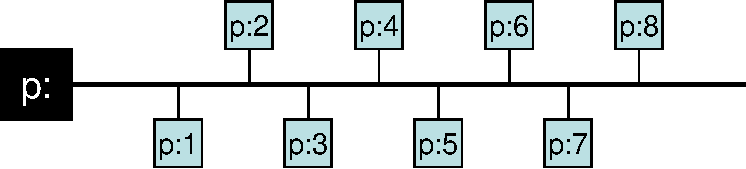
\includegraphics[width=0.5\textwidth]{Figures/iplink-crop.pdf} %	** if .eps or .pdf, don't need extension}
\caption{An IP link {\tt p:} with network prefix $p$. \emph{IP addresses of nodes in this IP link have the structure {\tt p:i}$/[p]$, for $0 < i < 2^{[p]}$.}}
\label{f:iplink}
\end{figure}

\paragraph{Forwarding rule}

When source and destination of a packet do not belong to the same IP link, routers receiving the packet compare the IP address of the destination to the prefixes stored in the routing table, and forward the packet through the network \glslink{interface}{interface} corresponding to the prefix showing the {\em longest prefix match}, this is, the prefix in the routing table for which a bigger number of bits are coincident with those from the network prefix of the IP address of the packet destination. %This is the {\em closest} prefix towards the destination, according to the IP closeness notion and the IP ordering criterion over the addressing space induced by the definition of IP link.

%\begin{definition}[IP Partial Order]
%Given two IP addresses $IPA_1/m_1$ and $IPA_2/m_2$ ($m_i$ being the prefix length of IP address $IPA_i$), $IPA_1 \subseteq_{IP} IPA_2$ if and only if:
%\begin{enumerate}[(i)]
%\item $IPA_1 \otimes NM_{\textrm{ max}\{m_1, m_2\}} = IPA_2 \otimes NM_{\textrm{ max}\{m_1, m_2\}}$ 
%\item $m_1 \geq m_2$
%\end{enumerate}
%where $NM_k$ is the netmask of $k$ bits and $\otimes$ denotes the bitwise AND operation.
%\end{definition}

%\begin{remark}
%The relationship $\subseteq_{IP}$ satisfies trivially the axioms of partial order:
%	\begin{itemize}
%	\item \emph{Reflexivity}: $IP_a \subseteq_{IP} IP_a$.
%	\item \emph{Antisymmetry}: $IP_a \subseteq_{IP} IP_b, IP_b \subseteq_{IP} IP_a \Longrightarrow IP_a \sim_{IP} IP_b$, that is, $IP_a$ and $IP_b$ are in the same IP link.
%	\item \emph{Transitivity}: $IP_a \subseteq_{IP} IP_b, IP_b \subseteq_{IP} IP_c \Longrightarrow IP_a \subseteq_{IP} IP_c$.
%	\end{itemize}
%\end{remark}

%For routing of packets for which the IP link of the destination is not the same as the IP link of the source, the IP addressing model provides a simple rule for making forwarding decisions. Given the IP address of the packet’s destination, a router should forward the packet through the \glslink{interface}{interface} providing connection to the IP network closest to the destination, where the notion of {\em closeness} is as follows:

%\begin{definition}[IP Closeness]
%Given an IP address $IPA_d/m_d$ and two IP addresses $IPA_1/m_1$ and $IPA_2/m_2$, $IPA_1/m_1$ is \emph{IP-closer} to $IPA_d/m_d$ than to $IPA_2/m_2$ if:
%	\begin{itemize}
%	\item $IPA_d \subseteq_{IP} IPA_1$ and $IPA_d \not\subseteq_{IP} IPA_2$, or
%	\item $IPA_d \subseteq_{IP} IPA_1 \subseteq_{IP} IPA_2$ (which is equivalent to $|m_1| \geq |m_2|$, for the case $IPA_d \subseteq_{IP} IPA_{1,2}$).
%	\end{itemize}
%\end{definition}

%According to this decision criterion, routers select send a given IP packet to the \glslink{interface}{interface} whose IP address has the \emph{longest prefix match} with respect to the IP packet destination. 

%\begin{remark}
%Note that the longest prefix match is only guaranteed to exist if and only if the router has a \emph{default route} ({\tt 0.0.0.0/0} in IPv4, {\tt ::/0} in IPv6).
%\end{remark}

\subsection{Main Routing Techniques}
\label{ss:routing}
%
Two types of routing techniques currently dominate \cite{interconnections}: {\em link-state} routing and {\em distance-vector} routing (with the variant of {\em path-vector} routing). The main protocols used historically and currently in the Internet are based on these techniques.
%
\paragraph{Link-State Routing} Routers advertise the status of their links (link-state) to the whole network. Link status may include information about the type of link (broadcast, point-to-point...), the link communication capabilities (one-directional, bi-directional, link cost) or the routers to which communication is available through this link. This way, every router in the network receives the link-state of other routers in the network, maintains information about the whole network topology and is therefore able to locally compute network-wide shortest paths, usually by way of Dijkstra's algorithm \cite{dijkstra59}. 
	\begin{itemize}
	\item Some examples of this approach are the Open Shortest Path First (OSPF, RFCs 2328 and 5340 \cite{rfc2328,rfc5340}) and the Intermediate System to Intermediate System (IS-IS, RFC 1142 \cite{rfc1142}) protocols, as well as the Optimized Link State Routing protocol (OLSR, RFC 3626 \cite{rfc3626}).
	\end{itemize}

\paragraph{Distance-Vector Routing} A router shares information from its routing table only with its neighbors, indicating \emph{distances} and next hops towards reachable destinations. Neighbor distance is defined according to the current \glslink{metric}{\em link metric}, which maps links between routers with estimations of the cost of sending packets through them, represented by scalar values. By receiving the routing tables of all its neighbors, which in turn have been shared with the neighbors of the neighbors, a router is able to identify, for each advertised destination, the neighbor that provides shortest distance and select it as next hop. Distance-vector protocols mostly use the distributed Bellman-Ford algorithm \cite{bellman58,ford56} to identify network-wide shortest paths. 
	\begin{itemize}
	\item The Routing Information Protocol (RIP, RFCs 1058 \cite{rfc1058}, 2080 \cite{rfc2080} and 2453 \cite{rfc2453}) is a prominent example of this family.
	\end{itemize}

\paragraph{Path-vector routing} It is based on the same principle as distance-vector routing, a router advertises to its neighbors the paths to all reachable destinations. Each path is described by indicating the routers that are traversed. This way, local distribution of locally maintained paths enables all routers in the network to build routes to all possible destinations. 
	\begin{itemize}
	\item The most prominent example of this family of protocols is the Border Gateway Protocol (BGP, RFC 1771 \cite{rfc1771}). \\
	\end{itemize}

% -------------
The link-state algorithm requires that every single router has storage and computational capacity to compute locally the shortest-path tree of the network, based on the information received from every other routers, and extract from that tree the next-hop towards every destination in the network. Distance-vector algorithms only require that each router updates the distance-vectors received from their neighbor to infer its own vector of distance vector and select its next-hops. \ \\ \ \\
%
Due to their computational simplicity, distance-vector protocols were used in the early stages of the Internet. They were gradually replaced by link-state protocols as the ARPANET grew bigger and more complex, due to problems such as the well-known count-to-infinity problem \cite{tanenbaum} (which appears in the original distance-vector algorithm, but does not appear on path-vector protocols). Poor scalability and slow convergence properties of distance-vector with respect to link-state algorithms were also major reasons to switch from one technique to the other \cite{interconnections}.

\begin{itemize}
\item The network reaction to a link failure illustrates the differences between link-state and distance-vector algorithms in terms of convergence. In distance-vector algorithms, once a router detects such a failure, it updates the cost of its route towards the lost neighbor and sends the new vector of distances to its neighbors. Neighbors receive this update and {\em recompute} the cost of the affected route, and then transmit in turn their new vectors. Propagation of topology changes is thus slower than in link-state algorithms, in which a router detecting the failure of the link towards one of its neighbors {\em floods} an updated topology description which is directly forwarded over the network, without delays caused by route re-computation in intermediate routers \cite{interconnections}.
\end{itemize}
% ------------------

Routing protocols for wired networks used to be {\em proactive} or table-driven, in which next hop to any possible destination is stored in a table.  With the emergence of wireless networks and, more generally, more dynamic networking architectures coping with more scarce (shared) bandwith, {\em reactive} routing protocols were then designed and deployed, in which routes were only computed upon request (on-demand).

\paragraph{Proactive routing} Routers collect and periodically disseminate topology information over the network; this enables them to maintain proactively (\emph{i.e.}, regardless on whether they are used) routes towards all destinations. This way, routers are able to forward packets at any time to any destination in the network.

\paragraph{Reactive routing} A router calculates a route to a destination only when it receives packets addressed to that destination and the routing table does not provide a next hop towards it. In this case, the router triggers a {\em route discovery} process by disseminating a Route Request (RREQ) packet through the network. The route discovery process terminates when the requested destination or another router knowing a valid route towards the destination reply to the requesting router.  
	\begin{itemize}
	\item Dynamic Source Routing (DSR, RFC 4728 \cite{rfc4728}) or Ad hoc On-Demand Distance Vector (AODV, RFC 3561 \cite{rfc3561}), both used in spontaneous wireless networks, are examples of reactive routing protocols. \\
	\end{itemize}

Proactive maintenance of next hops to every possible destination in the table requires a constant exchange of control traffic in the network, but enables routers to forward packets immediately after receiving them. Reactive protocols adapt the control traffic to the data traffic requirements: when there is no traffic to route, or the traffic follows known paths, a mostly negligible amount of control traffic (very low or even zero, depending on the protocol) is needed. When a router receives packets to be sent to a destination for which no route is known, the router needs to address a route discovery process over the network -- such a discovery process is costly in terms of overhead, and leads to significant delays in the forwarding.

\paragraph{Other routing approaches} Some other approaches have been explored for routing over spontaneous wireless networks. In some cases, they rely on additional assumptions about properties and capabilities of the involved devices. If nodes' position is available (for instance, by way of GPS), {\bf geographical routing} approaches are possible: in these protocols, a packet is forwarded to the relay getting closer to the final destination. The Greedy Perimeter Stateless Routing (GPSR) protocol \cite{gpsr} was the first protocol exploring this principle.

%\begin{tabular}{|c||c|c|}
%\hline
%    		& Proactive 		& Reactive  	\\ \hline\hline
%Link-State 	& OSPF, IS-IS, OLSR 	& 		\\ \hline
%Distance-Vector	& RPL, RIP, BGP 	& AODV, LOAD	\\ \hline
%\end{tabular}


%\subsubsection{Other Approaches}

%\begin{itemize}
%\item Opportunistic routing. ExOR.
%\item Source routing. DSR.
%\end{itemize}

\subsection{The Internet Routing Architecture}
\label{ss:irarq}

In terms of routing, the Internet is organized as a set of interconnected internetworks, denominated {\em Autonomous Systems} (see Figure \ref{f:ass}). The networks in each Autonomous System are under the same administrative control, and are assumed to perform routing inside the AS {\em autonomously} from the rest of networks in the Internet. The formal definition of an AS is as follows:

\begin{definition}[Autonomous System]
``An \emph{Autonomous System (AS)} is a connected group of one or more IP prefixes [internetwork] run by one or more network operators which has a SINGLE and CLEARLY DEFINED routing policy" \cite{rfc1930}, the term ``routing policy" denoting the way that routing information is exchanged between (but not within) Autonomous Systems. In the interior of an AS, ``routers may use one or more interior routing protocols, and sometimes several sets of \glslink{metric}{metrics}" \cite{rfc1812}.
\end{definition}

\begin{figure}[htb]	% H-must be here or [htb]
\centering
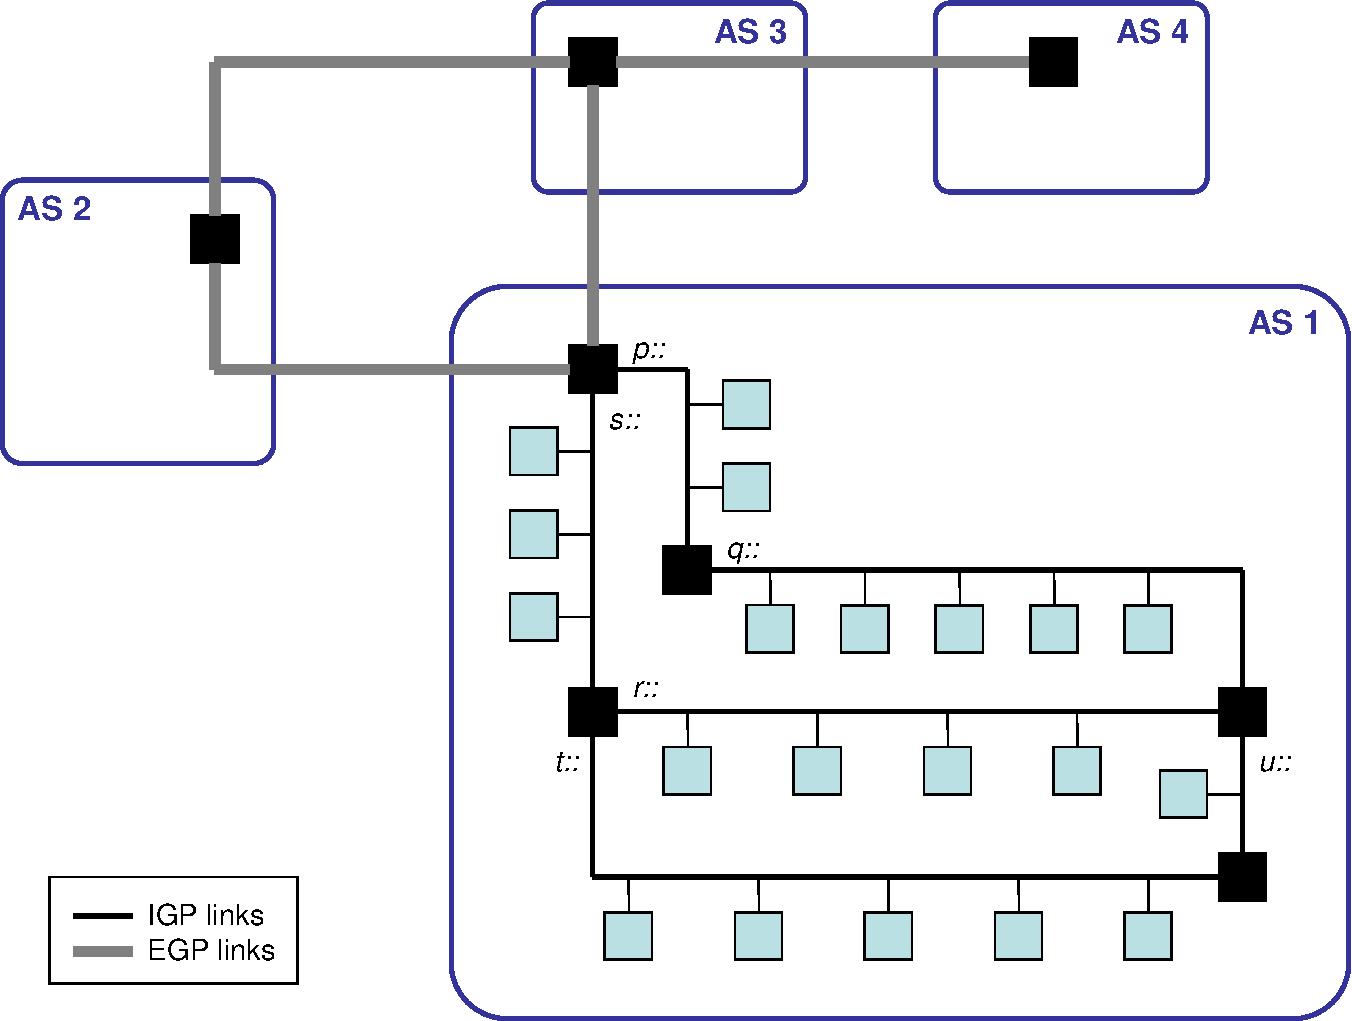
\includegraphics[width=0.8\textwidth]{Figures/ass-crop.pdf} %	** if .eps or .pdf, don't need extension}
\caption{Connection of different Autonomous Systems.}
\label{f:ass}
\end{figure}

The distinction between routing inside an Autonomous System (intra-AS or intra-domain routing) and routing between different ASes (inter-AS or inter-domain routing) leads to two different types of routing protocols: 

\begin{enumerate}[(i)]
\item {\em Interior Gateway Protocols} (IGPs), for route discovery and maintenance within an Autonomous System. Intra-domain routing is mostly performed by way of link-state protocols; the most significant link-state routing protocol for TCP/IP networks in the Internet are the Open Shortest Path First protocol (OSPF, \cite{rfc2328, rfc5340}, described in section \ref{s:wospf}) and the Integrated IS-IS, an IP variant of the Intermediate Systems to Intermediate Systems (IS-IS) protocol (see \cite{rfc1195}).
\item {\em Exterior Gateway Protocols} (EGPs), for route acquisition and information exchange between different Autonomous Systems. The current standard protocol for inter-domain routing is the path-vector Border Gateway Protocol (BGP, \cite{rfc1771}).
\end{enumerate}


